\begin{XeClass}{NativeS3FileSystem}
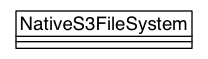
\includegraphics[width=\textwidth]{cdig/NativeS3FileSystem.png}
     
 <p>
 A \emph{FileSystem} for reading and writing files stored on
 <a href="http://aws.amazon.com/s3">Amazon S3</a>.
 Unlike \emph{org.apache.hadoop.fs.s3.S3FileSystem} this implementation
 stores files on S3 in their
 native form so they can be read by other S3 tools.
 A note about directories. S3 of course has no "native" support for them.
 The idiom we choose then is: for any directory created by this class,
 we use an empty object "#{dirpath}_$folder$" as a marker.
 Further, to interoperate with other S3 tools, we also accept the following:
 - an object "#{dirpath}/' denoting a directory marker
 - if there exists any objects with the prefix "#{dirpath}/", then the
 directory is said to exist
 - if both a file with the name of a directory and a marker for that
 directory exists, then the *file masks the directory*, and the directory
 is never returned.
 </p>



\end{XeClass}
